\documentclass[12pt, a4paper]{article}
\usepackage{a4wide}

\usepackage[utf8]{inputenc}
\usepackage[spanish]{babel}

\usepackage{color}
\usepackage{url}
\definecolor{lnk}{rgb}{0, 0, 0.4}
\usepackage[colorlinks = true, linkcolor = lnk, citecolor = black,urlcolor = black]{hyperref}

\usepackage{./otros/ulem}
\usepackage{./otros/caratula}

\usepackage{amssymb}
\usepackage{pdfpages}
\usepackage{framed}

\usepackage[small, bf, labelformat = empty]{caption}	
\usepackage{subfig}
\usepackage{float}

\usepackage{enumitem}
\usepackage{listings}

\usepackage{makeidx}
\makeindex

\begin{document}
  %Carátula
	\titulo{Trabajo Práctico 1}
	\subtitulo{}
	\fecha{17 de Julio de 2013}
	\materia{Bases de Datos}
	\integrante{Agustina Ciraco}{630/06}{agusciraco@gmail.com}	
	\integrante{Nadia Heredia}{589/08}{heredianadia@gmail.com}
	\integrante{Pablo Antonio}{290/08}{pabloa@gmail.com}
	\integrante{Vanesa Stricker}{159/09}{vanesastricker@gmail.com}  
	\maketitle

	% Índice
	\small
	\newpage \printindex \tableofcontents
	\normalsize

	\newpage
	\section{Introducci\'on}

En este trabajo pr\'actico, analizaremos el impacto de las diferentes
estrategias para manejar los buffer pools.
Nos concentraremos en el m\'odulo \textit{Buffer Manager}.

\vspace*{0.3cm}

Las diferentes estrategias que consideraremos son

\begin{itemize}
    \item
            un solo buffer
    \item
            múltiples buffers (distribución de Oracle)    
\end{itemize}

\vspace*{0.3cm}

Veremos las ventajas y desventajas de cada uno seg\'un la situaci\'on.

\subsection{Formato}

\vspace*{0.3cm}

En primera instancia, presentaremos una breve explicación
del uso de los múltiples buffer, luego se explicar\'an ciertos 
detalles de implementaci\'on, as\'i como tambi\'en las decisiones 
tomadas durante el desarrollo.

\vspace*{0.3cm}

Por \'ultimo, daremos nuestras conclusiones.


	\newpage
	\section{Diagrama Entidad-Relaci\'on}

% -----------------------------------------------------------------------------
\thispagestyle{empty}
  \begin{figure}[H] \centering
    \subfloat[der]
    {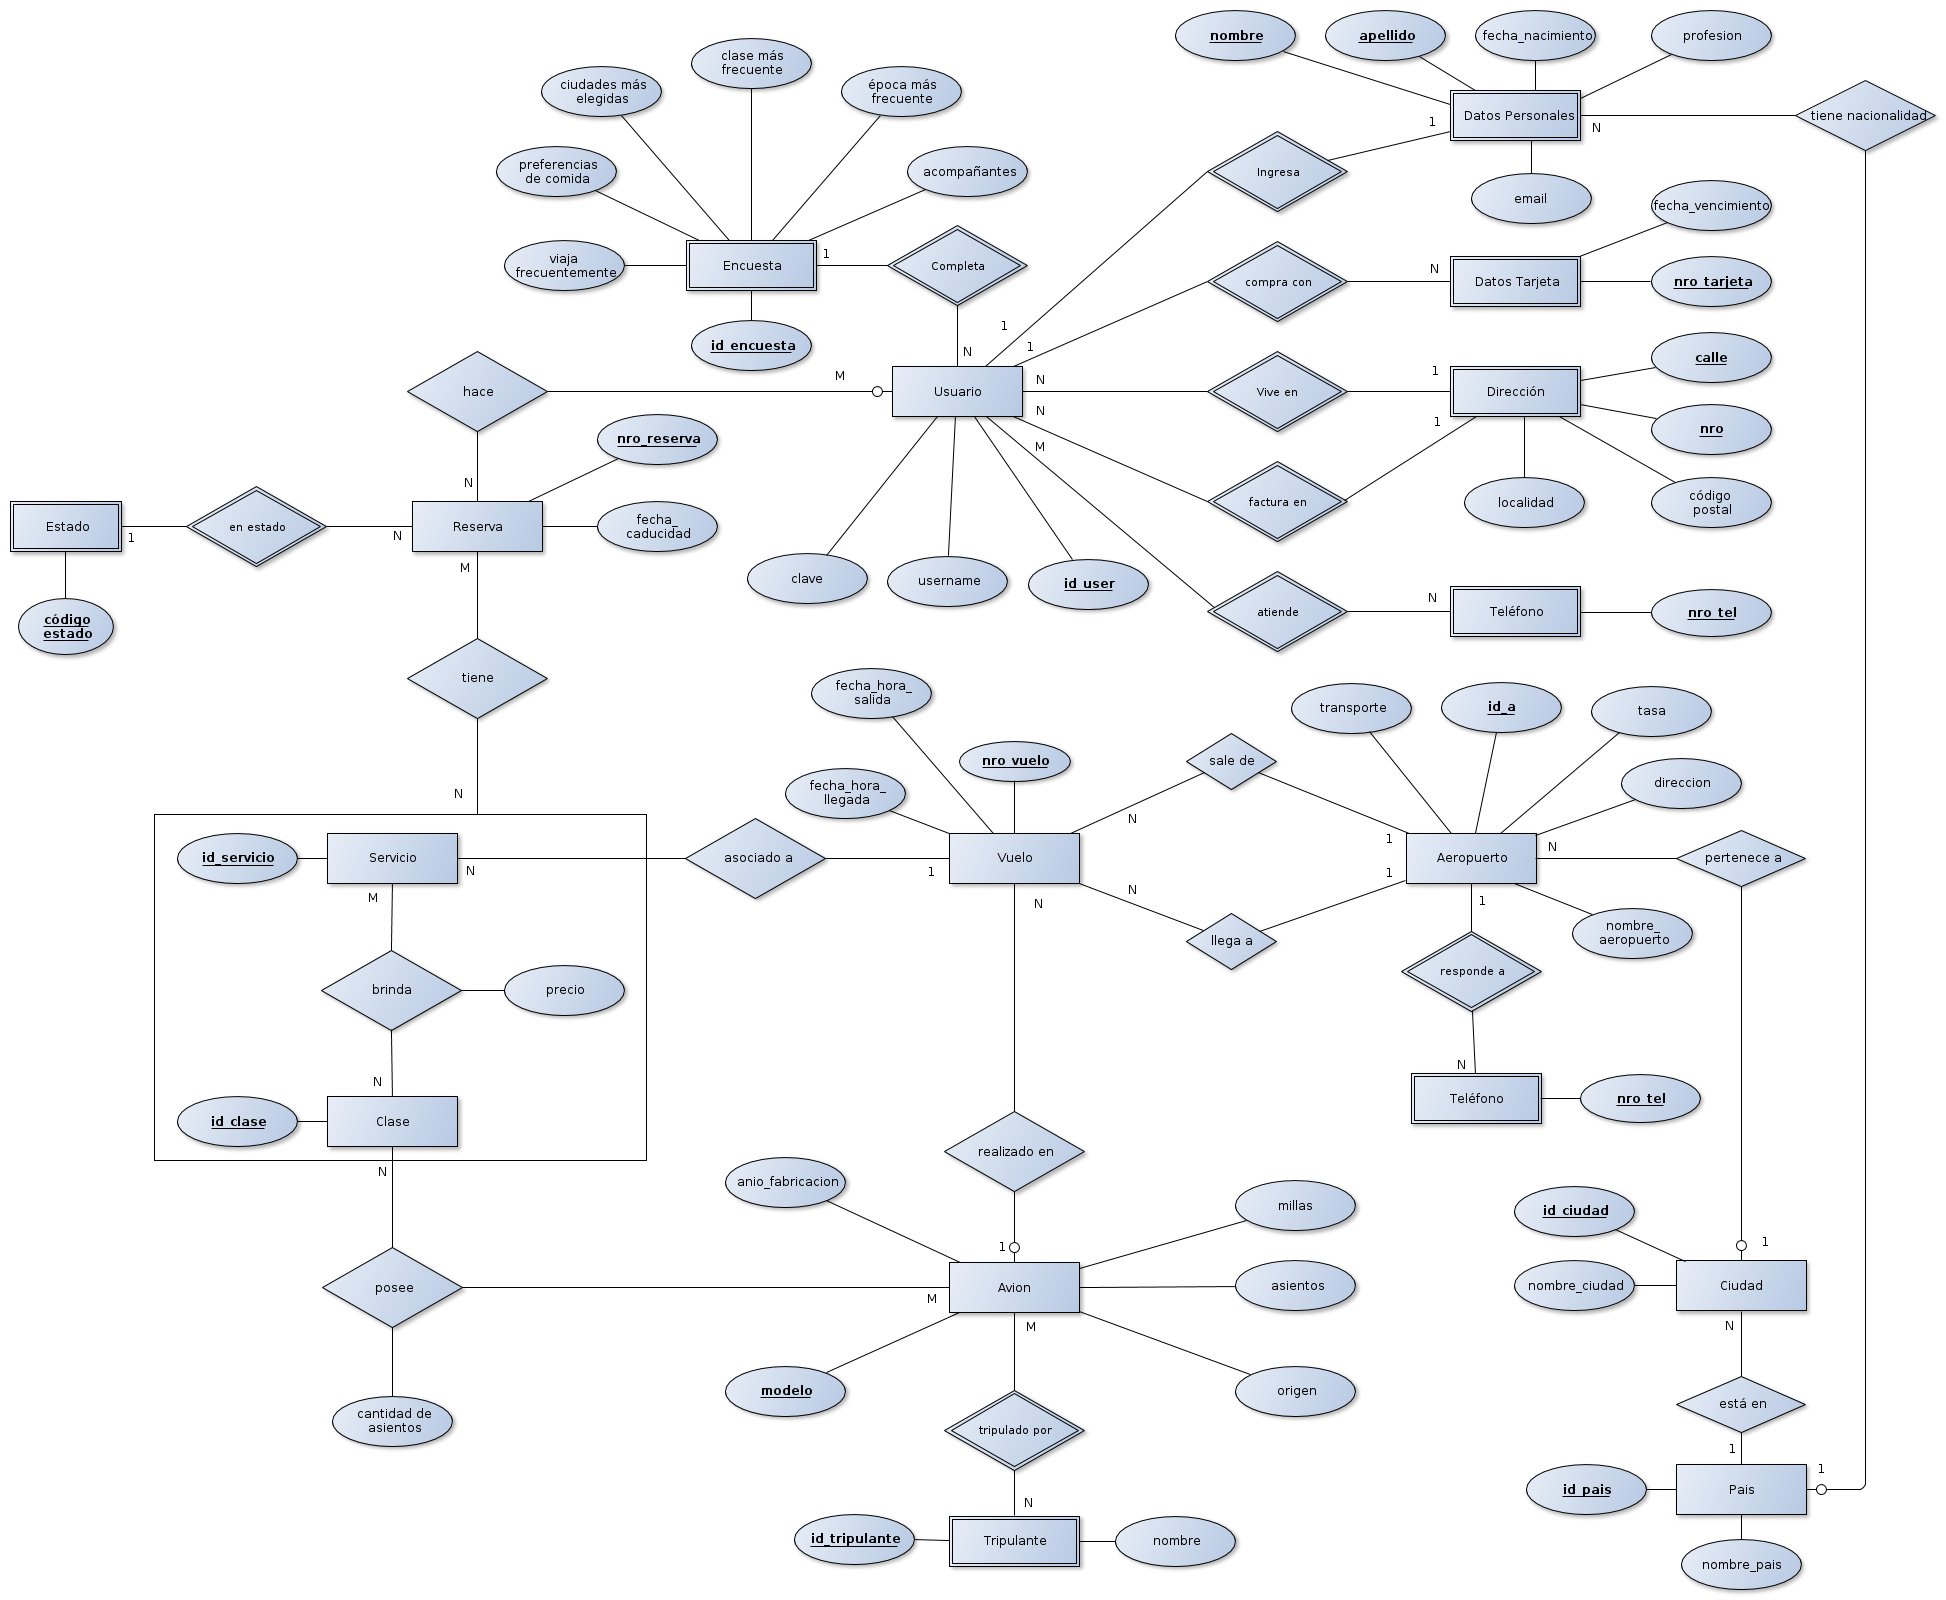
\includegraphics[width=\linewidth]{./img/der.png}}
    {}
  %\hspace*{6cm}
  \end{figure} 

% -----------------------------------------------------------------------------

\subsection{Aclaraciones y Restricciones}
  \begin{itemize}
    \item Consideramos que una reserva puede tener varios estados, estos son
          \begin{itemize}
            \item   Realizada
            \item   Cancelada
            \item   Confirmada
          \end{itemize}

          Las reservas realizadas pueden cancelarse o confirmarse.
          Es necesario confirmar una reserva para poder viajar.
          Para simplificar, suponemos que todos los usuarios con reservas
          confirmadas realizan efectivamente el viaje.
    
    \item La aerolínea ofrece servicios de viaje, y cada usuario realiza una
          reserva sobre pares de servicio-clase.
          De esta forma vemos la cantidad de asientos que está reservando por
          cada clase para un servicio.
          Cada servicio especifica la fecha y el horario del viaje. Además 
          tiene asociado un avión, que es el avión con el que se realizará
          el viaje.
          A la vez un servicio está vinculado con un vuelo. Un vuelo es
          un conjunto de servicios sin especificar. Es decir, un vuelo indica 
          que dias de la semana se brindarán servicios de un aeropuerto origen 
          a uno destino.
          Así, por ejemplo, un servicio podría ser:
          ``Un vuelo de Aeropuerto de origen Ezeiza- Buenos Aires, Aeropuerto 
          destino Newark-New Jersey el día 26/04/2013, 15:00hs, Primera Clas''.
          En cambio, un ejemplo de vuelo es:
         ``Vuelos de Aeropuerto origen Barajas-Madrid, Aeropuerto destino 
          JFK-New York, los días martes y jueve''.
	
    \item Consideramos que los mensajes que el sistema le envía a los usuarios
          no son lo suficientemente relevantes para el problema que queremos
          modelar.
          
    \item Una reserva que se encuentra en estado Realizada, está asociada con un
    	  servicio cuya fecha y hora de salida es anterior a la fecha actual.
    	  
	\item La suma de la cantidad de asientos por clase en un avión (en la 
		  interrelación se distribuyen en) es igual a lo que indica el 
		  atributo asientos de la entidad avión.
	
	\item Este modelo no contempla la posibilidad de que la aerolinea cancele un
		  vuelo. Con lo cual todo vuelo existente es efectuado.
            
  \end{itemize}
	\newpage
	\section{Modelo Relacional}

% Notación
\begin{framed} \centering
  \underline{primary key} \hspace*{3cm}
  \dotuline{foreign key}
\end{framed}

\vspace*{0.5cm}
\noindent
$\mathbf{Usuario}$(\underline{id\_user}, username, clave, nombre, apellido)
\begin{itemize}
	\item $FK = \{(nombre, apellido, calle, nro)\}$
	\item $PK = \{id\_user\}$
	\item $CK = \{id\_user, (nombre, apellido)\}$
	\item $Usuario.nombre$ y $Usuario.apellido$ deben estar en una misma fila
		en $DatosPersonales.nombre$ y $DatosPersonales.apellido$
	\item $Usuario.calle$ y $Usuario.nro$ deben estar en una misma fila
		en $Direccion.calle$ y $Direccion.nro$

\end{itemize}

% Debiles de Usuario

\vspace*{0.5cm}
\noindent
$\mathbf{Encuesta}$(\underline{\dotuline{id\_user}, id\_encuesta},
	viaja\_frecuentemente, preferencias\_de\_comida, ciudades\_elegidas,
	clase\_mas\_frecuente, epoca\_mas\_frecuente, acompaniantes)
\begin{itemize}
	\item $FK = \{id\_user\}$
	\item $PK = CK = \{(id\_user, id\_encuesta)\}$
	\item $Encuesta.id\_user$ debe estar en $Usuario.id\_user$
\end{itemize}

\vspace*{0.5cm}
\noindent
DatosPersonales(\underline{\dotuline{id\_user}, nombre, apellido}, email,
					profesión, fecha\_nacimiento)
\begin{itemize}
	\item $FK = \{id\_user\}$
	\item $PK = CK = \{(id\_user, nombre, apellido\}$
	\item $DatosPersonales.id\_user$ debe estar en $Usuario.id\_user$
\end{itemize}

\vspace*{0.5cm}
\noindent
DatosTarjeta(\underline{\dotuline{id\_user}, nro\_tarjeta}, fecha\_vencimiento)
\begin{itemize}
	\item $FK = \{id\_user\}$
	\item $PK = CK = \{(id\_user, nro\_tarjeta\}$
	\item $DatosTarjeta.id\_user$ debe estar en $Usuario.id\_user$
\end{itemize}

% Como distinguimos las dos relaciones???

\vspace*{0.5cm}
\noindent
Direccion(\underline{\dotuline{id\_user}, calle, nro}, localidad,
					código postal)
\begin{itemize}
	\item $FK = \{id\_user\}$
	\item $PK = CK = \{(id\_user, calle, numero)\}$
	\item $Direccion.id\_user$ debe estar en $Usuario.id\_user$
\end{itemize}

\vspace*{0.5cm}
\noindent
Atiende(\underline{\dotuline{id\_user, nro\_tel}})
\begin{itemize}
	\item $FK = \{id\_user, nro\_tel\}$
	\item $PK = CK = \{(id\_user, nro\_tel)\}$
	\item $Atiende.id\_user$ debe estar en $Usuario.id\_user$
	\item $Atiende.nro\_tel$ debe estar en $Telefono.nro\_tel$
\end{itemize}

\vspace*{0.5cm}
\noindent
Telefono(\underline{\dotuline{id\_user}, nro\_tel})
\begin{itemize}
	\item $FK = \{id\_user\}$
	\item $PK = CK = \{(id\_user, nro\_tel)\}$
	\item $Telefono.id\_user$ debe estar en $Usuario.id\_user$
\end{itemize}


\vspace*{0.5cm}
\noindent
Reserva(\underline{nro\_reserva}, fecha\_caducidad, \dotuline{codigo\_estado})
\begin{itemize}
	\item $FK = \{estado\}$
	\item $PK = CK = \{nro\_reserva\}$
	\item $Reserva.codigo\_estado$ debe estar en $Estado.codigo\_estado$
\end{itemize}

\vspace*{0.5cm}
\noindent
Estado(\underline{codigo\_estado}, descripcion)
\begin{itemize}
	\item $FK = \emptyset$
	\item $PK = CK = \{codigo\_estado\}$
\end{itemize}

\vspace*{0.5cm}
\noindent
Servicio(\underline{id\_servicio}, fecha\_salida, fecha\_llegada,
	hora\_salida, hora\_llegada, \dotuline{nro\_vuelo, modelo})
\begin{itemize}
	\item $FK = \{nro\_vuelo, modelo\}$
	\item $PK = CK = \{id\_servicio\}$
	\item $Servicio.nro\_vuelo$ debe estar en $Vuelo.nro\_vuelo$
	\item $Servicio.modelo$ debe estar en $Avion.modelo$
\end{itemize}

\vspace*{0.5cm}
\noindent
Vuelo(\underline{nro\_vuelo}, \dotuline{aeropuerto\_salida},
	\dotuline{aeropuerto\_llegada})
\begin{itemize}
	\item $FK = \{aeropuerto\_salida, aeropuerto\_llegada\}$
	\item $PK = CK = \{nro\_vuelo\}$
	\item $Vuelo.aeropuerto\_salida$ debe estar en $Aeropuerto.id\_a$
	\item $Vuelo.aeropuerto\_llegada$ debe estar en $Aeropuerto.id\_a$
\end{itemize}

\vspace*{0.5cm}
\noindent
Avion(\underline{modelo}, anio\_fabricacion, millas, asientos, origen)
\begin{itemize}
	\item $FK = \emptyset$
	\item $PK = CK = \{modelo\}$
\end{itemize}


\vspace*{0.5cm}
\noindent
Tripulante(\underline{id\_tripulante}, nombre)
\begin{itemize}
	\item $FK = \emptyset$
	\item $PK = CK = \{id\_tripulante\}$
\end{itemize}


\vspace*{0.5cm}
\noindent
TripuladoPor(\underline{id\_tripulante, modelo})
\begin{itemize}
	\item $FK = \{id\_tripulante, modelo\}$
	\item $PK = CK = \{(id\_tripulante, modelo)\}$
	\item $TripuladoPor.id\_tripulante$ debe estar en
		$Tripulante.id\_tripulante$
	\item $TripuladoPor.modelo$ debe estar en $Avion.modelo$
\end{itemize}

\vspace*{0.5cm}
\noindent
Pais(\underline{id\_pais}, nombre\_pais)
\begin{itemize}
	\item $FK = \emptyset$
	\item $PK = CK = \{id\_pais\}$
\end{itemize}


\vspace*{0.5cm}
\noindent
Ciudad(\underline{id\_ciudad}, nombre\_ciudad, \dotuline{id\_pais})
\begin{itemize}
	\item $FK = \{id\_pais\}$
	\item $PK = CK = \{id\_ciudad\}$
	\item $Ciudad.id\_pais$ debe estar en $Pais.id\_pais$
\end{itemize}

\vspace*{0.5cm}
\noindent
TelefonoAeropuerto(\underline{nro\_tel, \dotuline{id\_a}})
\begin{itemize}
	\item $FK = \{id\_a\}$
	\item $PK = CK = \{(nro\_tel, id\_a\}$
	\item $TelefonoAeropuerto.id\_a$ debe estar en $Aeropuerto.id\_a$
\end{itemize}


\vspace*{0.5cm}
\noindent
Aeropuerto(\underline{id\_a}, tasa, direccion, transporte, nombre\_aeropuerto,
	\dotuline{id\_ciudad})
\begin{itemize}
	\item $FK = \{id\_ciudad\}$
	\item $PK = CK = \{id\_a\}$
	\item $Aeropuerto.id\_ciudad$ debe estar en $Ciudad.id\_ciudad$
\end{itemize}

% \newpage
\subsection{Restricciones}
\begin{itemize}
  \item
  
  \item
\end{itemize}

\subsection{Aclaraciones}
\begin{itemize}
  \item

\end{itemize}

	\newpage
	% \section{Consultas}

A continuación se presentan las consultas implementadas en SQL.

\subsection*{Consulta 1}

Mediante SQL escribir una consulta para obtener el nombre, apellido y número identificatorio
de aquellos pasajeros que han viajado a todos los países cubiertos por la línea aérea en los
últimos 5 años.


\begin{small}
\begin{verbatimtab}[2]

SELECT dp.nombre, dp.apellido, u.id_user
FROM Usuario u, DatosPersonales dp
WHERE NOT EXISTS
(
    SELECT p.id_pais, p.nombre
    FROM Vuelo v1, Aeropuerto a1, Ciudad c1, Pais p
    WHERE (v1.a_salida = a1.id_a or v1.a_llegada = a1.id_a)
    AND a1.id_ciudad = c1.id_ciudad
    AND c1.id_pais = p.id_pais
    AND NOT EXISTS
    (
	      SELECT *
	      FROM Hace h, Reserva r, Tiene t, Servicio s, Vuelo v, 
		      Aeropuerto a, Ciudad c, Estado e
	      WHERE u.id_user = h.id_user 
	      AND h.id_reserva = r.id_reserva 
	      AND r.id_reserva = t.id_res 
	      AND t.id_serv = s.id_servicio
	      AND s.id_vuelo = v.id_vuelo 
	      AND (v.a_llegada = a.id_a or v.a_salida = a.id_a) 
	      AND a.id_ciudad = c.id_ciudad 
	      AND c.id_pais = p.id_pais
	      AND r.id_estado = 3
	      AND ((s.salida >= date_sub(now(), interval 5 year)) 
		      OR (s.llegada >= date_sub(now(), interval 5 year)))  
    )
)
AND u.id_user = dp.id_user

\end{verbatimtab}
\end{small}

\newpage

\subsection*{Consulta 2}

Obtener un reporte que como mínimo contenga: Todos los códigos identificatorios de los
aeropuertos, un periodo de tiempo de la forma año/mes, la cantidad de pasajeros que
ascendieron y descendieron en ese aeropuerto durante el periodo. El reporte debe estar
ordenado por la cantidad total de personas que viajaron. Y debe ser ejecutado para un rango
de fechas. Aclaración: dependiendo del rango de fechas, para un mismo aeropuerto pueden
aparecer varios periodos distintos.

\begin{small}
\begin{verbatimtab}[2]

\end{verbatimtab}
\end{small}


\newpage

\subsection*{Consulta 3}

Controlar mediante alguna restricción que un usuario no pueda realizar reservas que se
superpongan en el tiempo. La única excepción que se permite consiste en que un usuario
puede realizar a lo sumo 2 reservas para la misma fecha de viaje entre los mismos
aeropuertos de origen y destino, siempre que la fecha de partida no se encuentre dentro de
los próximos 7 días.

\begin{small}
\begin{verbatimtab}[2]
CREATE TRIGGER chequear_reservas_superpuestas
BEFORE INSERT ON Tiene
FOR EACH ROW
begin
	IF EXISTS (
		SELECT h1.id_reserva, h1.id_user
		FROM Hace h1, Servicio s1, Usuario u1, Reserva r1
		WHERE h1.id_user = u1.id_user AND
			h1.id_reserva = r1.id_reserva AND
			NEW.id_res = r1.id_reserva AND
			NEW.id_serv = s1.id_servicio
			AND EXISTS(
			    SELECT s2.salida
			    FROM Servicio s2, Tiene t2, Reserva r2, Hace h2
			    WHERE h2.id_user = u1.id_user
				AND h2.id_reserva <> h1.id_reserva
				AND h2.id_reserva = r2.id_reserva
				AND t2.id_res = r2.id_reserva
				AND t2.id_serv = s2.id_servicio
				AND s2.salida = s1.salida
				AND s1.id_servicio <> s2.id_servicio
				AND s2.salida NOT IN (
					    (SELECT s3.salida
					    FROM Reserva r3, Hace h3, Tiene t3, Servicio s3, Usuario u3, Vuelo v3
					    WHERE r3.id_reserva = h3.id_reserva
						    AND r3.id_reserva = t3.id_res
						    AND u3.id_user = h3.id_user
						    AND t3.id_serv = s3.id_servicio
						    AND s3.id_vuelo = v3.id_vuelo
						    AND s3.salida IN (
								    SELECT s4.salida
								    FROM Servicio s4, Hace h4, Tiene t4, Reserva r4, Vuelo v4
								    WHERE r4.id_reserva <> r3.id_reserva
									    AND h4.id_reserva = r4.id_reserva
									    AND h4.id_user = h3.id_user
									    AND r4.id_reserva = t4.id_res
									    AND t4.id_serv = s4.id_servicio
									    AND s4.id_vuelo = v4.id_vuelo
									    AND v4.a_salida = v3.a_salida
									    AND v4.a_llegada = v4.a_llegada
									    AND datediff(s4.salida, now()) > 7)
								    ) 
							    )
	)) THEN
		SIGNAL SQLSTATE '45000'
			SET MESSAGE_TEXT = 'No se puede insertar la reserva';
	END IF;
end;
\end{verbatimtab}
\end{small}


Para poder imponer esta restricción, usamos un trigger, que cuando ocurre el evento: 
insertar en la tabla Tiene (tabla que relaciona las reservas con los servicios), se fija
que la reserva a la cual está asociada esta tabla no tenga como fecha de salida de vuelo
la misma fecha de salida de otras reservas del mismo usuario, salvo que la fecha de partida
del vuelo no sea dentro de la próxima semana. En caso de que tengta la misma fecha de salida
se dispara una excepción inexistente de manera tal que no se concreta la operación.

\newpage

\subsection*{Consulta 4}

Para las reservas superpuestas que se permiten en el punto anterior, se debe contar con una
funcionalidad que cancele una de las reservas duplicadas (la más económica) cuando la
fecha de partida se encuentre dentro de los próximos 7 días.


\begin{small}
\begin{verbatimtab}[2]
delete
from Reserva r1
where r1.id_reserva IN (
	select r2.id_reserva
	from Reserva r2, Tiene t, Servicio s, Hace h, Usuario u, Vuelo v, Brinda b
	where t.id_res = r2.id_reserva
	and t.id_serv = s.id_servicio
        and h.id_reserva = r2.id_reserva
        and h.id_user = u.id_user
        and s.id_vuelo = v.id_vuelo     
        and s.salida IN (
                select s2.salida
                from Servicio s2, Tiene t2      
                where s2.id_servicio = t2.id_serv 
                and t2.id_res = r1.id_reserva)

        and s.llegada IN ( 
                select s3.llegada
                from Servicio s3, Tiene t3      
                where s3.id_servicio = t3.id_serv 
                and t3.id_res = r1.id_reserva)
        and v.a_salida IN ( 
                select v4.a_salida
                from Servicio s4, Tiene t4, Vuelo v4
                where s4.id_servicio = t4.id_serv 
                and t4.id_res = r1.id_reserva
                and s4.id_vuelo = v4.id_vuelo)

	and v.a_llegada IN ( 
		select v5.a_llegada
		from Servicio s5, Tiene t5, Vuelo v5
		where s5.id_servicio = t5.id_serv
		and t5.id_res = r1.id_reserva
		and s5.id_vuelo = v5.id_vuelo)
	group by b.precio
	having min(b.precio)
)
\end{verbatimtab}
\end{small}


\newpage

\subsection*{Consulta 5}

Restricción adicional: Restricción que no permite modificar el estado de una reserva a realizada 
si la fecha de la reserva es posterior a la fecha actual


\begin{small}
\begin{verbatimtab}[2]
create trigger chequear_fechas_correctas
BEFORE UPDATE ON Reserva
FOR EACH ROW
begin
    IF NEW.id_estado = 3 THEN
        IF EXISTS (
            SELECT 1
            FROM Servicio s, Tiene t
            WHERE
                s.id_servicio = t.id_serv AND
                t.id_res = r.id_reserva AND
                (datediff(now(), s.salida) < 0) AND
                (datediff(now(), s.llegada) < 0)
        ) THEN
            SIGNAL SQLSTATE '45000'
                SET MESSAGE_TEXT =
                    'No se puede cambiar el  estado de la reserva';
        END IF;
    END IF;
end;
\end{verbatimtab}
\end{small}

El estado
	%\section{Suposiciones Generales}
	\begin{itemize}
    \item     

    \item  

	\end{itemize}

	% \newpage
  %%\section{Modelo F\'isico - Funcionalidades Implementadas}
\section{Modelo F\'isico}

\noindent
Para el modelo f\'isico elegimos utilizar 
% my-sql en un servidor online, que usa php.

\section{Modelo F\'isico - Funcionalidades Pedidas}

%\subsection{Restricciones}
%\subsection{Funcionalidades Implementadas}

\subsection{Stored Procedures}

\noindent
Para ejecutar el c\'odigo de los stored procedures se realiza lo siguiente

\vspace*{0.5cm}
\noindent
\textbf{Ejercicio 1} call ejercicio\_1 ()\\
\textbf{Ejercicio 2} call ejercicio\_2()\\
\textbf{Ejercicio 3} call ...

\newpage
\subsubsection{Proc 1.}

\begin{verbatim}
delimiter $$
create procedure ejercicio_1()
begin

end;
$$
delimiter ;
\end{verbatim}

\vspace*{0.5cm}
\noindent
Aclaraciones .......


\newpage
\subsubsection{Proc 2.}

\begin{verbatim}
delimiter $$
create procedure ejercicio_2()
begin

end;
$$
delimiter ;
\end{verbatim}

\newpage
\subsection{Triggers - Restricciones}

\subsubsection{}

\begin{verbatim}
delimiter $$
create trigger nombre
before insert 
begin

end;
$$
delimiter ;
\end{verbatim}

	% \newpage
	% \section{Modelo F\'isico - Funcionalidades Adicionales}

%\newpage
\subsection{Triggers - Restricciones}
\subsubsection{Trigger 1.}

\begin{verbatim}
delimiter $$
create trigger nombre
before insert 
begin

end;
$$
delimiter ;
\end{verbatim}

\subsubsection{Trigger 2.}
 
\begin{verbatim}
delimiter $$
create trigger nombre
before insert 
begin

end;
$$
delimiter ;
\end{verbatim}
	% \newpage
	% \section{Dificultades Encontradas}

\noindent
% Al encarar el desarrollo de las restricciones del modelo f\'isico, 
% nos encontramos que my-sql tiene algunas limitaciones.

\vspace*{0.5cm}
\noindent
% No permite devolver m\'ultiples filas para un store procedure.
% S\'olo permite un trigger para una misma acci\'on para una misma tabla.

	% \section{Conclusiones}



\end{document}
